\documentclass[main.tex]{subfiles}
\begin{document}

\chapter{Oefeningen}
\label{cha:oefeningen}

\section{Kansruimten}
\label{sec:kansruimten}
\begin{oef}
  Een bepaalde vorm van kanker (in het beginstadium) treft 3 Belgen op
  1000. Men heeft een zeer betrouwbare maar dure test ontwikkeld die
  deze vorm van kanker moet opsporen: niet- getroffen personen
  reageren positief op de test in 5\% van de gevallen (vals
  alarm). Slechts 2\% van de personen die deze vorm van kanker hebben
  in zijn beginstadium, reageren negatief (niet-detecteren van de
  kanker). Is het rendabel voor de staat om elke Belg te testen?\\\\
  We beginnen met definities van notatie:
  \begin{itemize}
  \item Als we willekeurig een Belg kiezen is de kans $\frac{3}{1000}$ dat die kanker heeft: $P(K) = \frac{3}{1000}$.
  \item Als we een Belg zonder kanker testen is de kans $\frac{5}{100}$ dat de test postief uitslaagt: $P(P|G) = \frac{5}{100}$.
  \item Als we een Belg met kanker testen is de kans $\frac{2}{100}$ dat de test negatief uitslaagt: $P(N|K) = \frac{2}{100}$.
  \item We zoeken nu de kans dat een Belg kanker heeft, gegeven dat de test positief uitslaagt: $P(K|P)$
  \end{itemize}
  Merk eerst op dat de kans dat een test enkel positief op negatief kan uitslaan, en een belg enkel al dan niet kanker kan hebben.
  \[ P(P) + P(N) = 1 \wedge P(K) + P(G) = 1 \]
  Er is dus ook het volgend verband:\stref{st:rekenregel-afhankelijkheid-partitie}
  \[ P(P|\ \cdot) + P(N|\ \cdot) = 1  \wedge P(K|\ \cdot) + P(G|\ \cdot) = 1 \]
  Hierna kunnen we de wet van de totale kans gebruiken:
  \[
  \begin{array}{rl}
    P(P)
    &= P(K)P(P|K) + P(G)P(P|G)\\
    &= P(K)(1-P(N|K) + (1-P(K))P(P|G)\\
    &= \frac{3}{1000}\left(1-\frac{2}{100}\right) + \left(1-\frac{3}{1000}\right)\frac{5}{100}\\
    &= 5.279 \% \\
  \end{array}
  \]
  We gebruiken de stelling van Bayes\stref{st:bayes} om $P(K|P)$ te berekenen.
  \[
  \begin{array}{rl}
    P(K|P)
    &= \frac{P(K)P(P|K)}{P(K)P(P|K) + P(G)P(P|G)}\\
    &= \frac{P(K)\left(1-P(N|K)\right)}{P(K)\left(1-P(N|K)\right) + (1-P(K))P(P|G)}\\
    &= \frac{\frac{3}{1000}\left(1-\frac{2}{100}\right)}{\frac{3}{1000}\left(1-\frac{2}{100}\right) + \left(1-\frac{3}{1000}\right)\frac{5}{100}}\\
    &= 5.567 \%
  \end{array}
  \]
\end{oef}

\begin{oef}
  Er wordt een vraag gesteld en je mag kiezen tussen $m$ antwoorden waarvan er \'e\'en het juiste antwoord is. De kans dat je het antwoord weet, is gelijk aan $p$. Toon aan dat de voorwaardelijke kans dat je het antwoord wist, gegeven dat je juist geantwoord hebt, gelijk is aan $x$:
  \[ x = \frac{mp}{mp + 1 - p} \]
  \begin{proof}
    Definities:
    \begin{itemize}
    \item Noem $P(J)$ de kans dat je de vraag juist had.
      \[ P(J) + P(F) = 1 \]
    \item Noem $P(W)$ de kans dat je het antwoord wist.
      \[ P(W) + P(N) = 1 \]
    \item Veronderstel dat, wanneer je het antwoord niet weet, je altijd wilekeurig gokt en het anders altijd juist hebt.
      \[ P(J|W) = 1 \]
    \end{itemize}
    Omdat je willekeurig gokt wanneer je het antwoord niet weet, is het volgende ook gegeven:
    \[ P(J|N) = \frac{1}{m} \]
    We zoeken nu $P(W|J)$.
    We gebruiken hiervoor de stelling van Bayes:
    \[
    \begin{array}{rl}
      P(W|J)
      &= \frac{P(W)P(J|W)}{P(W)P(J|W) + P(N)P(J|N)}\\
      &= \frac{p}{p + (1-p)\left(\frac{1}{m}\right)}\\
      &= \frac{mp}{mp + 1-p}\\
    \end{array}
    \]
  \end{proof}
\end{oef}

\begin{oef}
  Zij $\Omega = \{1,2,3,4,5,6\}$.
  Beschouw $C= \{\{1,2,3,4\},\{3,4,5,6\}\}$ en zij $\sigma(C)$ de $\sigma$-algebra voortgebracht door $C$.
  Bepaal $\sigma(C)$.\\\\
  $\emptyset$ en $\Omega$ moeten zeker tot $\sigma(C)$ behoren.\deref{de:sigma-algebra}\stref{st:lege-verzameling-in-sigma-algebra}
  \[ \{\emptyset, \Omega\} \subset \sigma(C)\]
  Het complement van alle elementen in $C$ moet tot $\sigma(C)$ behoren.
  \[ \{ \{5,6\},\{1,2\}\} \subset \sigma(C) \]
  De unie en de doorsnede van elke twee elementen in $C$ moet tot $\sigma(C)$ behoren.
  \[ \{3,4\} \in \sigma(C) \]
  \[ \{1,2,5,6\} \in \sigma(C) \]
  \[ \sigma(C) = \{ \{1,2\},\{3,4\},\{5,6\},\{1,2,3,4\},\{3,4,5,6\},\{1,2,5,6\},\{1,2,3,4,5,6\} \} \]
\end{oef}

\begin{oef}
  Zij $\Omega = \{1,2,3,4,5,6\}$.
  Noem $\mathcal{A} = \mathcal{P}(\Omega)$.
  Beschouw $P$:
  \[
  P:\ \mathcal{A} \rightarrow \mathcal{R}:\
  \left\{
    \begin{array}{rcl}
      \emptyset &\mapsto &0\\
      \{1\} &\mapsto &\frac{r}{6}\\
      \{2\} &\mapsto &\frac{6-r}{6}\\
      \{i\} &\mapsto & 0 \text{ met } i \in \{3,4,5,6\}\\
      A &\mapsto &\sum_{x \in A} P(x)\\
    \end{array}
  \right.
  \]
  Is $P$ een kansmaat?\\\\
  Ja:
  \begin{proof}
    We gaan de definierende eigenschappen van een kansmaat af:
    \begin{itemize}
    \item $P(\Omega) = \frac{r}{6} + \frac{6-r}{6} = 1$
    \item $\forall A \in \mathcal{A}:\ P(A) \ge 0$
    \item De laatste eigenschap geldt vanuit de definitie van $P$.
    \end{itemize}
  \end{proof}
\end{oef}

\begin{oef}
  Twee studenten spreken af om samen te gaan eten in de Alma ergens tussen 12u en 13u. Op
  de dag zelf vergeten ze echter het exacte tijdstip van deze afspraak. Onderstel dat beiden nu
  lukraak arriveren tussen twaalf en \'e\'en en dat ze slechts $10$ minuten aan de ingang blijven staan
  wachten totdat de andere persoon eventueel opdaagt. Wat is de kans dat ze op deze manier
  samen de Alma binnengaan?
  \begin{figure}[H]
    \centering
    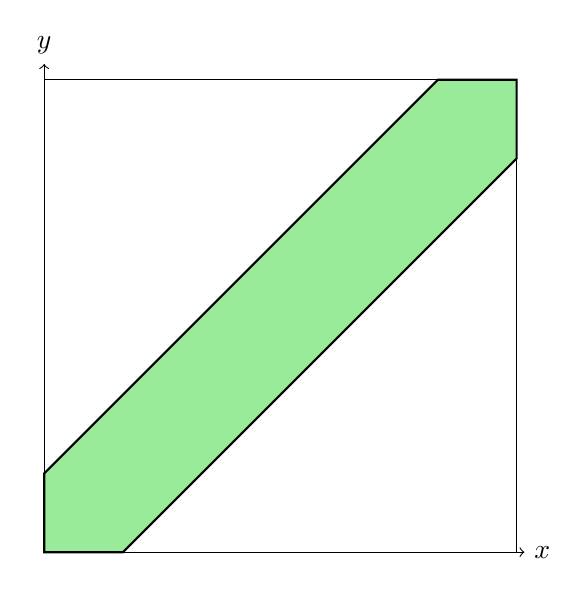
\begin{tikzpicture}
      \draw[->] (0,0) -- (6.1,0) node[right] {$x$};
      \draw[->] (0,0) -- (0,6.2) node[above] {$y$};
      \draw (0,6) -- (6,6) node {};
      \draw (6,0) -- (6,6) node {};
      \draw (0,1) -- (5,6) node {};
      \draw (1,0) -- (6,5) node {};
      \filldraw[thick,fill=green!80!black,fill opacity=0.4] (0,0) -- (1,0) -- (6,5) -- (6,6)  -- (5,6) -- (0,1) -- cycle;
    \end{tikzpicture}
    \caption{Het universum}
  \end{figure}
  Noem $x\in \interval{0}{60}$ de aankomsttijd van de eerste student.
  Noem $y\in \interval{0}{60}$ de aankomsttijd van de tweede student.
  De gebeurtenis waarin de twee studenten elkaar tegenkomen noemen we $A$ en duiden we aan op de grafiek.
  \[ A = \{ (a,b) \mid |a-b| \le 10 \}\]
  We berekenen de gevraagde kans nu als de verhouding van de oppervlakken.
  \[ P(A) = 1 - \frac{\frac{2\cdot 50 \cdot 50 }{2 \cdot}}{60\cdot 60} = \frac{11}{36} \]
\end{oef}

\begin{oef}
  Beschouw een blad met parallelle lijnen op afstand $d$ van elkaar.
  Gooi lukraak een naald van lengte $L$ (veronderstel $L < d$) op het blad.
  Wat is de kans dat de naald minstens \'e\'en van de evenwijdige lijnen snijdt?
  \begin{figure}[H]
    \centering
    \begin{tikzpicture}[scale=2]
      \draw (0,0) -- (3,0);
      \draw (0,2) -- (3,2);
      \draw[<->] (.1,0) -- (.1,2) node[left] {$d$};
      \draw (1,.5) -- (2,2) node[above] {$\frac{L}{2}$};
      \draw (1,1.25) -- (2,1.25);
      \draw[->] (1.75,1.25) arc (0:30:.5cm);
      \draw (1.75,1.30) node[right] {$\alpha$};
    \end{tikzpicture}
  \end{figure}
  We definieren eerst $\Omega$:
  \[ \Omega = \left\{ (a,\alpha) \mid a \in \interval[open right]{0}{d} \wedge \alpha \in \interval[scaled, open right]{-\frac{\pi}{2}}{ \frac{\pi}{2}} \right\} \]
  \begin{figure}[H]
    \centering
    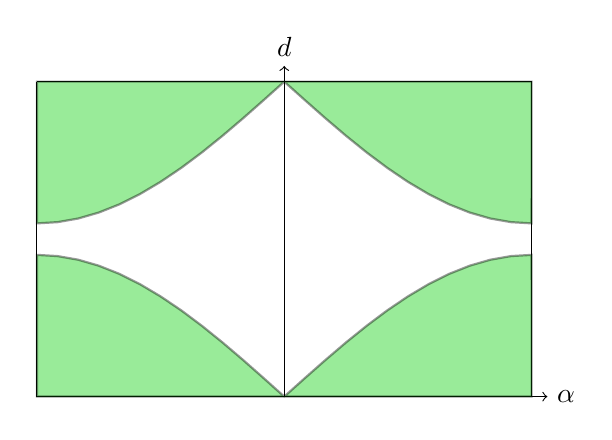
\begin{tikzpicture}[scale=2]
      \draw[->] (-pi/2,0) -- (pi/2+0.1,0) node[right] {$ \alpha $};
      \draw[->] (0,0) -- (0,2.1) node[above] {$d$};
      \draw (-pi/2,0) -- (-pi/2,2) node {};
      \draw (pi/2,0) -- (pi/2,2) node {};
      \draw (-pi/2,2) -- (pi/2,2) node {};
      %\draw[scale=1,domain=-pi/2:pi/2,smooth,variable=\al,red] plot ({\al},{1.8*abs(sin(deg(\al)))});
      %\draw[scale=1,domain=-pi/2:pi/2,smooth,variable=\al,blue] plot ({\al},{1.8-1.8*abs(sin(deg(\al)))});
      \filldraw[thick,fill=green!80!black,opacity=.4] (-pi/2,0) --  plot [domain=-pi/2:pi/2] ({\x},{1.8/2*abs(sin(deg(\x)))}) -- (pi/2,0) -- cycle;
      \filldraw[thick,fill=green!80!black,opacity=.4] (-pi/2,2) --  plot [domain=-pi/2:pi/2] ({\x},{2-1.8/2*abs(sin(deg(\x)))}) -- (pi/2,2) -- cycle;
    \end{tikzpicture}
    \caption{Het universum}
  \end{figure}
  De gebeurtenis dat een naald een lijn overlapt is aangeduid.
  Het is de unie van het deel van het universum waar $a \ge d-\frac{L}{2}\sin(\alpha)$ geldt en het deel waar $a \le \frac{L}{2}\sin(\alpha)$ geldt.
  \[ \left\{ (a,\alpha) \mid (a, \alpha) \in \Omega) \wedge a \ge d-\frac{L}{2}\sin(\alpha) \vee a \le \frac{L}{2}\sin(\alpha) \right\}\]
  We berekenen de oppervlakte van het gekleurde deel dus als volgt:
  \[ 1-2\left(\int_{0}^{\frac{\pi}{2}} d-\frac{L}{2}\sin(\alpha)\ d\alpha- \int_{0}^{\frac{\pi}{2}}\frac{L}{2}\sin(\alpha)\ d\alpha \right) = \frac{2L}{\pi d} \]
\end{oef}

\begin{oef}
  Een vaas bevat $5$ rode en $10$ zwarte ballen.
  Trek lukraak een bal uit de vaas en noteer de kleur.
  Na elke trekking wordt de bal teruggelegd en wordt er \'e\'en extra bal van dezelfde kleur toegevoegd.
  Beantwoord de volgende vragen:
  \begin{itemize}
  \item Gegeven dat de eerste $n$ ballen allemaal zwart zijn, bereken de kans dat de $n+1$-ste bal ook zwart is en bereken de limiet:
    \[ \lim_{n \rightarrow +\infty}P(Z_{n+1}|Z_{1} \cap Z_{2} \cap \dotsb \cap Z_{n}) \]
  \item Gegeven dat de tweede tot en met de $n+1$-ste bal allemaal zwart zijn, bereken de kans dat de eerste getrokken bal zwart was en bereken de limiet:
    \[ \lim_{n \rightarrow +\infty}P(Z_{1}| Z_{2} \cap Z_{3} \cap \dotsb \cap Z_{n+1}) \]
  \end{itemize}
  Voor de trekking zijn er $5$ rode en $10$ en zwarte ballen.
  Wanneer er $r$ rode en $z$ zwarte ballen zijn is de kans $p$ dat er een zwarte bal getrokken word als volgt te berekenen:
  \[ p = \frac{z}{z+r} \]
  \begin{itemize}
  \item  Na $n$ zwarte ballen zijn er $10+n$ zwarte ballen en nog steeds $5$ rode ballen.
    \[ P(Z_{n+1}|Z_{1} \cap Z_{2} \cap \dotsb \cap Z_{n}) = \frac{10+n}{5+10+n} = \frac{10+n}{15+n} \]
    \[ \lim_{n \rightarrow +\infty}P(Z_{n+1}|Z_{1} \cap Z_{2} \cap \dotsb \cap Z_{n}) = \lim_{n \rightarrow +\infty}\frac{10+n}{15+n} = 1 \]
  \item
    Bekijk eerst ook nog de vorige situatie waarbij de eerste bal rood is:
    \[ P(R_{1}) = \frac{5}{15}\]
    \[ P(Z_{2} | R_{1}) = \frac{10}{6+10} \]
    \[ P(Z_{n+1}|R_{1} \cap Z_{2} \cap \dotsb \cap Z_{n}) = \frac{10+(n-1)}{6+10+(n-1)} = \frac{9+n}{15+n} \]
    Gebruik dan zo'n beetje elke rekenregel.
    \[
    \begin{array}{rl}
      P(Z_{1}| Z_{2} \cap Z_{3} \cap \dotsb \cap Z_{n+1})
      &= \frac{P(Z_{1}\cap Z_{2} \cap Z_{3} \cap \dotsb \cap Z_{n+1})}{P(Z_{2} \cap Z_{3} \cap \dotsb \cap Z_{n+1})}\\
      &= \frac{P(Z_{1})P(Z_{2}|Z_{1})P(Z_{3}|Z_{2}\cap Z_{1}) \cdot\ \dotsb\ \cdot P(Z_{n+1}|Z_{1} \cap Z_{2} \cap \dotsb \cap Z_{n}) }{P(Z_{1} \cap Z_{2} \cap Z_{3} \cap \dotsb \cap Z_{n+1})+P(R_{1} \cap Z_{2} \cap Z_{3} \cap \dotsb \cap Z_{n+1})}\\
      &= \frac{\prod_{i=1}^{n}\frac{10+i}{15+i} }{\prod_{i=1}^{n}\frac{10+i}{15+i}+P(R_{1} \cap Z_{2} \cap Z_{3} \cap \dotsb \cap Z_{n+1})}\\
      &= \frac{\prod_{i=1}^{n}\frac{10+i}{15+i} }{\prod_{i=1}^{n}\frac{10+i}{15+i}+\frac{5}{15}\prod_{i=1}^{n}\frac{9+i}{15+i}}\\
      &= \frac{\prod_{i=1}^{n}\frac{10+i}{15+i} }{\frac{10+n}{10}\prod_{i=1}^{n}\frac{9+i}{15+i}+\frac{5}{15}\prod_{i=1}^{n}\frac{9+i}{15+i}}\\
      &= \frac{\frac{10+n}{10}\prod_{i=1}^{n}\frac{9+i}{15+i} }{\left(\frac{10+n}{10}+\frac{5}{15}\right)\prod_{i=1}^{n}\frac{9+i}{15+i}}\\
      &= \frac{\frac{10+n}{10}}{\left(\frac{10+n}{10}+\frac{5}{15}\right)}\\
      &= \frac{10+n}{500+50n}\\
    \end{array}
    \]
    \[ \lim_{n \rightarrow +\infty}P(Z_{n+1}|Z_{1} \cap Z_{2} \cap \dotsb \cap Z_{n}) = \lim_{n \rightarrow +\infty}\frac{10+n}{500+50n} = 1 \]
  \end{itemize}
\end{oef}

\section{Stochastische veranderlijken}
\label{sec:stoch-verand}

\begin{oef}
  Om naar de campus te komen moet ik de bus nemen in het station van Leuven. De wachttijd (in minuten) heeft dichtheidsfunctie: $f$
  \[
  f: \mathbb{R} \rightarrow \mathbb{R}:\ x \mapsto
  \left\{
    \begin{array}{rl}
      \frac{c}{5}x & \text{ als } x\in \interval[open right]{0}{5}\\
      c \left(2-\frac{1}{5}x\right) & \text{ als } x\in \interval[open right]{5}{10}\\
      0 & \text{ elders }
    \end{array}
  \right.
  \]

  \begin{itemize}
  \item Bepaal $c$ zodat $f$ een dichtheidsfunctie is.\\
    Opdat $f$ een dichtheidsfunctie zou zijn moet de volgende integraal $1$ zijn.
    \[
    \begin{array}{rl}
      \int_{-\infty}^{+\infty}f(x)\ dx 
      &= \int_{0}^{10}f(x)\ dx \\
      &= \int_{0}^{5}\frac{c}{5}\ dx + \int_{5}^{10}c\left(2-\frac{1}{5}\right)\ dx\\
      &= \frac{25c}{10} + 10c - \frac{75c}{10}\\
      &= \frac{50c}{10}
    \end{array}
    \]
    $c$ moet dus $\frac{1}{5}$ zijn.
    De functie is dus de volgende:
    \[
    f: \mathbb{R} \rightarrow \mathbb{R}:\ x \mapsto
    \left\{
      \begin{array}{rl}
        \frac{x}{25} & \text{ als } x\in \interval[open right]{0}{5}\\
        \frac{2}{5}-\frac{1}{25}x & \text{ als } x\in \interval[open right]{5}{10}\\
        0 & \text{ elders }
      \end{array}
    \right.
    \]
  \item Wat is de kans dat de totale wachttijd ten hoogste drie minuten is?
    \[
    \begin{array}{rl}
      P(X \le 3)
      &= \int_{-\infty}^{3}f(x)\ dx\\
      &= \int_{0}^{3}\frac{x}{25}\ dx\\
      &= \frac{9}{50}
    \end{array}
    \]
  \item Wat is de kans dat de totale wachttijd ten hoogste acht minuten is?
    \[
    \begin{array}{rl}
      P(X \le 8)
      &= \int_{-\infty}^{8}f(x)\ dx\\
      &= \int_{0}^{5}\frac{x}{25}\ dx + \int_{5}^{8}\left(\frac{2}{5}-\frac{1}{25}x\right)\ dx\\
      &= \frac{25}{50} + \frac{6}{5} - \frac{39}{50}\\
      &= \frac{23}{25}
    \end{array}
    \]
  \item Wat is de kans dat de totale wachttijd tussen drie en acht minuten ligt\\
    \[ P(3 \le X \le 8) = P(X \le 8) - P(X \le 3) = \frac{23}{25}-\frac{9}{50} = \frac{35}{50} = \frac{7}{10} \]
  \item Wat is de kans dat de totale wachttijd kleiner is dan twee minuten of groter is dan zes\\
    minuten?
    \[
    \begin{array}{rl}
      P(X \le 2 \vee X \ge 6)
      &= \int_{-\infty}^{2}f(x)\ dx + \int_{6}^{+\infty}f(x)\ dx\\
      &= \int_{0}^{2}\frac{x}{25}\ dx + \int_{6}^{10}\left(\frac{2}{5}-\frac{1}{25}x\right)\ dx\\
      &= \frac{1}{50}\left[x^{2}\right]_{0}^{2} + \frac{2}{5}\left[x\right]_{6}^{10}-\frac{1}{50}\left[x^{2}\right]_{6}^{10}\\
      &= \frac{4}{50} + \frac{8}{5} - \frac{100 -36}{50}\\
      &= \frac{2}{5}
    \end{array}
    \]
  \end{itemize}
\end{oef}

\begin{oef}
  Aan een bepaalde universiteit zijn er voor het tweede jaar burgerlijk-ingenieur $350$ studenten ingeschreven.
  Bij het begin van het academiejaar worden ze door lottrekking ingedeeld in $11$ groepen: $10$ groepen (genummerd van $1$ tot en met $10$) van dertig studenten en $1$ groep (groepsnummer $11$) van $50$ studenten.

  \begin{itemize}
  \item  E\'en van de studenten is Jan. Noem $X$ de grootte van de groep waarin deze student terecht komt.
    $X$ kan je aanzien als een toevalsvariabele. 
    Bepaal $E[X]$.\\\\
    Jan kan ofwel in een groep met $30$ studenten terecht komen, ofwel in een groep met $50$ studenten.
    \[ P(X=30) = \frac{10\cdot 30}{10 \cdot 30 + 1 \cdot 50} = \frac{300}{350} \quad\text{ en }\quad P(X=50) = \frac{1\cdot 50}{10 \cdot 30 + 1 \cdot 50} = \frac{50}{350} \]
    We kunnen nu $E[X]$ bepalen:
    \[ E[X] = 30 \cdot \frac{300}{350} + 50 \cdot \frac{50}{350} = \frac{11500}{350} = 32.85... \]
  \item  Men beschikt verder over $11$ assistenten: eveneens door lottrekking wordt aan ieder een groep toegewezen.
    Noem $Y$ de grootte van de groep die aan de oudste assistent wordt toegekend.
    Bepaal $E[Y]$.\\\\
    De oudste assistent kan eveneens ofwel aan een groep van $30$ studenten, ofwel aan een groep met $50$ studenten toegekend worden.
    \[ P(Y=30) = \frac{10}{11} \quad\text{ en }\quad P(X=50) = \frac{1}{11} \]
    We kunnen nu $E[Y]$ bepalen:
    \[ E[Y] = 30\frac{10}{11} + 50\frac{1}{11} = \frac{350}{11} = 31.81... \]
  \end{itemize}
\end{oef}

\begin{oef}
  Omdat het verkeer tussen twee steden $A$ en $B$ vaak gehinderd wordt door voertuigen die in panne staan, besluit de plaatselijke overheid maatregelen te nemen door een vliegende brigade van automecaniciens op te richten.
  Deze wil men laten opereren vanuit een basisstation ergens tussen de twee steden in (zeg in een punt $b$), zodat de gemiddelde verplaatsing van het nog op te richten station tot de bestuurder in panne minimaal is op lange termijn.
  Hierbij is het zo dat het volgende kansmodel de plaats $X$ tussen de $2$ steden waar een panne optreedt, het best weergeeft:
  \[
  f_{X}(x) = 
  \left\{
    \begin{array}{rl}
      \frac{x}{2} & \text{ als } 0 \le x \le 2\\
      0 & \text{ elders }
    \end{array}
  \right.
  \]
  Ter informatie: stad $A$ bevindt zich in de oorsprong en stad $B$ in het punt met als $x$-co\"ordinaat $2$.
  Bovendien komt $1$ eenheid overeen met $10$ kilometer.
  Er zijn nu twee zinvolle manieren denkbaar om uitdrukking te geven aan de verplaatsing die telkens moet gebeuren, namelijk: $|X-b|$ of $(X-b)^{2}$.
  Werken met $X-b$ is immers niet aangewezen aangezien je in dat geval een negatieve afstand kan uitkomen.
  \begin{itemize}
  \item Vindt $b \in \interval{0}{2}$ zodat $E[|X-b|]$ minimaal wordt.
    Bereken vervolgens $F_{X}(b)$.
    \[
    \begin{array}{rl}
      E[|X-b|]
      &= \int_{-\infty}^{+\infty}f_{X}(x)\ dx\\
      &= \int_{0}^{2}|x-b|\frac{x}{2}\ dx\\
      &= \int_{0}^{b}(b-x)\frac{x}{2}\ dx + \int_{b}^{2}(x-b)\frac{x}{2}\ dx\\
      &= \frac{1}{2}\left(\int_{0}^{b}(bx-x^{2})\ dx + \int_{b}^{2}(x^{2}-bx)\ dx\right)\\
      &= \frac{1}{2}\left(\int_{0}^{b}bx\ dx-\int_{0}^{b}x^{2}\ dx + \int_{b}^{2}x^{2}\ dx-\int_{b}^{2}bx\ dx\right)\\
      &=\frac{1}{2}\left(\frac{1}{2}[x^{2}]_{0}^{b}-\frac{1}{3}[x^{3}]_{0}^{b} + \frac{1}{3}[x^{3}]_{b}^{2}-\frac{1}{2}[x^{2}]_{b}^{2}\right)\\
      &= \frac{1}{2}\left(\frac{1}{2}b^{2}-\frac{1}{3}b^{3} + \frac{1}{3}(8-b^{3})-\frac{1}{2}(8-b^{2})\right)\\
      &= \frac{4}{3} + b - \frac{b^{3}}{6}\\
    \end{array}
    \]
    \[
    \begin{array}{cc}
      \frac{d}{db}\left(\frac{4}{3} + b - \frac{b^{3}}{6}\right) &= 0\\
      1 - \frac{b^{2}}{2} &= 0\\
      2 - b^{2} &= 0\\
      |b| &= \sqrt{2}\\
    \end{array}
    \]
    $E[|X-b|]$ is dus minimaal wanneer $b=\sqrt{2}$ geldt.
    We berekenen tenslotte $F_{X}(b)$ als volgt:
    \[ F_{X}(b) = \frac{b}{2} =\frac{\sqrt{2}}{2} \]
  \item Bereken $E[X]$.
    \extra{oefening}
  \item Vindt vervolgens $b \in \interval{0}{2}$ zodat $E[(X-b)^{2}]$ minimaal wordt.
    \extra{oefening}
  \end{itemize}
\end{oef}

\begin{oef}
  Veronderstel dat $n$ studenten, waaronder jezelf en een vriend(in), lukraak achter elkaar worden gezet.
  Noem $Y$ het aantal mensen dat tussen jullie twee in staat. $Y \
in \{ 0,1,\dotsc,n-2 \}$.
  Bewijs $E[Y] =\frac{n-2}{8}$.

\begin{proof}
    We bekijken eerst de mogelijkheden:
    \begin{itemize}
    \item Het totaal aantal manieren om $n$ mensen op een rij te zetten is $P_{n}=n!$.
    \item Het aantal manieren waarop we kunnen staan met $0$ mensen ertussen is $2(n-1) \cdot P_{n-2}$.
    \item Het aantal manieren waarop we kunnen staan met $1$ persoon ertussen is $2(n-2) \cdot P_{n-2}$.
    \item Het aantal manieren waarop we kunnen staan met $i$ mensen ertussen is $2(n-1-i) \cdot P_{n-2}$.
    \end{itemize}
    De factor stamt van het feit dat je jezel en je vriend(in) kan omwisselen, de factor $(n-1-i)$ komnt van het aantal plaatsen waar de groep met (en tussen) jou en je vrien(in) kan staan en de factor $P_{n-2}$ komt van het aantal manieren dat de andere mensen kunnen staan.
    \[ 
    \begin{array}{rl}
    E[Y]
    &= \sum_{i=0}^{n-2}i \cdot \frac{\left( 2(n-1-i) \cdot P_{n-2} \right)}{n!}\\
    &= \sum_{i=0}^{n-2}i \cdot \frac{\left( 2(n-1-i) \cdot (n-2)! \right)}{n!}\\
    &= \frac{2(n-2)!}{n!}\sum_{i=0}^{n-2}i \cdot (n-1-i)\\
    &= \frac{2(n-2)!}{n!}\sum_{i=0}^{n-2}(in- i-i^{2})\\
    &= \frac{2(n-2)!}{n!}\left(\sum_{i=0}^{n-2}in- \sum_{i=0}^{n-2}i-\sum_{i=0}^{n-2}i^{2}\right)\\
    &= \frac{2(n-2)!}{n!}\left((n-1)\sum_{i=0}^{n-2}i-\sum_{i=0}^{n-2}i^{2}\right)\\
    &= \frac{2(n-2)!}{n!}\left((n-1)\frac{n(n-1)}{2}-\frac{n(n-1)(2(n-1)+1)}{6}\right)\\
    &= \frac{2(n-1)!}{n!}\left(\frac{n(n-1)}{2}-\frac{n(2(n-1)+1)}{6}\right)\\
    &= \frac{2n!}{n!}\left(\frac{(n-1)}{2}-\frac{(2(n-1)+1)}{6}\right)\\
    &= \frac{3(n-1)-(2(n-1)+1)}{3}\\
    &= \frac{n-2}{3}\\
    \end{array}
    \]
\end{proof}
\begin{proof}
  Alternatief:\\
  Noem $X_{i}$ het aantal mensen in groep $G_{i}$:
  \begin{itemize}
  \item $G_{1}$: de mensen tussen jullie.
  \item $G_{2}$: de mensen links van beide.
  \item $G_{3}$: de mensen links van beide.
  \end{itemize}
  Elk van de $n-2$ mensen komt in \'e\'en van de drie groepen terecht en met dezelfde kans.
  \[ E(X_{1}) = E(X_{2}) = E(X_{3}) \]
  Bovendien geldt $X_{1}+X_{2}+X_{3}= n-2$.
  \[ n-2 = E(X_{1}+X_{2}+X_{3}) \]
  \[ n-2 = E(X_{1})+E(X_{2})+E(X_{3}) \]
  \[ n-2 = 3E(X_{1}) \]
  \[ \frac{n-2}{3} = E(X_{1}) \]
\end{proof}
\end{oef}

\begin{oef}
  Een kandidaat neemt deel aan een quiz waarbij opeenvolgende vragen gesteld worden. Hij mag
naar de volgende ronde overstappen als hij $50$ vragen juist beantwoord heeft. Om aan een saldo
van $50$ juiste antwoorden te komen, mag de kandidaat zich hoogstens $4$ keer vergissen. Bereken
de kans dat de kandidaat in de volgende ronde raakt, als men veronderstelt dat de kans om een
goed antwoord te geven $0.9$ bedraagt.\\\\
  Noem $X$ het aantal keer dat de kandidaat zich vergist voordat hij $50$ juiste antwoorden geeft.
  $X$ is dat negatief binomiaal verdeeld.
  \[ X \sim NB(r=50,p=0.9) \]
  We zoeken nu de volgende kans:
  \[ P(X \le 4) = P(X=0) + P(X=1) + P(X=2) + P(X=3) + P(X=4) \]
  \formularium{Binomiaalverdeling}{$P(X=k) = \binom{k+r-1}{k}p^{r}(1-p)^{k}$}
  \[
  \begin{array}{l}
    = \binom{49}{0}(0.9)^{50} + \binom{50}{1}(0.9)^{50}(0.1) + \binom{51}{2}(0.9)^{50}(0.1)^{2} + \binom{53}{3}(0.9)^{50}(0.1)^{3} + \binom{54}{4}(0.9)^{50}(0.1)^{4}\\
    = \cdots\\
    = 0.361447
  \end{array}
  \]
\end{oef}

\begin{oef}
  Het aantal eieren dat door een vogel gelegd wordt, is Poisson verdeeld met parameter $\lambda$.
  De kans dat een ei voor het uitbroeden vernietigd wordt, is $p$.
  Zoek de kans dat geen enkel ei uitgebroed wordt.\\\\
  Noem $X$ het aantal eieren dat gelegd worden.
  \[ X \sim P(\gamma) \]
  Noem $Y$ het aantal eieren dat uitgebroed worden.
  \[ Y | X = n \sim B(n,p) \]
  We zoeken nu de kans $P(Y=0)$, maar we kennen enkel $Y|X=n$, niet $Y$.
  \[ P(Y=0) = \sum_{k=0}^{+\infty}P(Y=0|X=k)P(X=k) \]
  \formularium{Poissonverdeling}{$P(X=k) = e^{-\lambda}\frac{\lambda^{k}}{k!}$}
  \formularium{Binomiaalverdeling}{$P(Y=k|X=n)=\binom{n}{k}p^{k}(1-p)^{n-k}$}
  \[
  \begin{array}{rl}
    P(Y=0)
    &= \sum_{k=0}^{+\infty}P(Y=0|X=k)P(X=k)\\
    &= \sum_{k=0}^{+\infty}\binom{k}{0}p^{k}(1-p)^{k-k}e^{-\lambda}\frac{\lambda^{k}}{k!}\\
    &= \sum_{k=0}^{+\infty}\frac{p^{k}\lambda^{k}e^{-\lambda}}{k!}\\
    &= e^{-\lambda} \sum_{k=0}^{+\infty}\frac{(p\lambda)^{k}}{k!}\\
    &= e^{-\lambda} e^{px}\\
    &= e^{-\lambda(1-p)}\\
  \end{array}
  \]
  \formularium{Formules bovenaan}{$e^{k} = \sum_{k=0}^{\infty}\frac{x^{k}}{k!}$}
\end{oef}

\begin{oef}
  Veronderstel dat de snelheid van auto's op een bepaald stuk weg normaal verdeeld is. Men
heeft experimenteel bepaald dat $5\%$ van de auto's trager dan $100$ km/u rijdt en dat $20\%$ van de
auto's sneller dan $130$ km/u rijdt. Hoeveel procent van de auto's gaat sneller dan $145$ km/u?\\\\
  Noem $X$ de snelheid van een auto.
  We gaan ervan uit dat $X$ normaal verdeeld is:
  \[ X \sim N(\mu,\sigma^{2}) \]
  We hebben de volgende gegevens over $X$...
  \[ P(X \le 100) = 0.05 \text{ en } P(X > 130) = 0.2 \]
  ... en zoeken de volgende kans:
  \[ P(X > 145) \]
  Omdat $X$ normaal verdeeld is, gelden deze kansen ook voor de $Z$-scores van deze snelheden.
  \[ 
  \left\{
    \begin{array}{rcl}
      P(X \le \frac{100-\mu}{\sigma}) &=& 0.05\\
      P(X \le \frac{130-\mu}{\sigma}) &=& 1-0.2\\
    \end{array}
  \right.
  \]
  \tabel{Standaard normale verdeling}{De waarde waarvoor $P(X \le a) = 0.05$ geldt is $a=-1.645$  (Onthoudt, de tabel is symmetrisch rond $0$.) en de waarde waarvoor $P(X \le b)$ geldt is $b=0.84$.}
  \[
  \left\{
    \begin{array}{rcl}
      \frac{100-\mu}{\sigma} &=& -1.645\\
      \frac{130-\mu}{\sigma} &=& 0.84\\
    \end{array}
  \right.
  \quad\longrightarrow\quad
  \left\{
    \begin{array}{rl}
      \mu &= 119.859\\
      \sigma &= 12.072\\
    \end{array}
  \right.
  \]
  We kunnen nu de gevraagde kans berekenen:
  \[ P(X > 145) = 1-P(X \ge 145) = 1-P\left(Z \le \frac{145-119.859}{12.072}\right) = 1-P(Z\le 2.082) = 0.019 \]
  \tabel{Standaard normale verdeling}{De waarde in de tabel bij $2.082$ is $0.981$.}
\end{oef}


\begin{oef}
  Een lognormale verdeling wordt voorgesteld als model om de $SO_{2}$ concentratie boven een bos te beschrijven.
  Stel dat de $SO_{2}$ concentratie gemiddelde $1.9$ en standaardafwijking $0.9$ heeft.
  Wat is de kans dat de concentratie op een gegeven moment tussen $5$ en $10$ ligt?\\\\
  Noem $X$ de $SO_{2}$ concentratie boven het bos.
  Noem $Y=\ln(X)$.
  We zoeken de volgende kans:
  \[ P( 5 \le X \le 10) \]
  We berekenen $\mu_{Y}$ en $\sigma_{Y}$ vanuit $\mu_{X}$ en $\sigma_{X}$:\\
  \formularium{Lognormale verdeling}{$\mu_{X} = e^{\mu_{Y} + \frac{\sigma_{Y}^{2}}{2}}$ en $\sigma_{X}^{2} = e^{2\mu_{Y} + \sigma_{Y}^{2}}\left(e^{\sigma_{Y}^{2}}-1\right)$}
  \[
  \left\{
    \begin{array}{rl}
      \mu_{X} &= e^{\mu_{Y} + \frac{\sigma_{Y}^{2}}{2}}\\
      \sigma_{X}^{2} &= e^{2\mu_{Y} + \sigma_{Y}^{2}}\left(e^{\sigma_{Y}^{2}}-1\right)\\
    \end{array}
  \right.
  \quad\longrightarrow\quad
  \left\{
    \begin{array}{rl}
      \mu_{X} &= 0.5407\\
      \sigma_{X} &= 0.4499\\
    \end{array}
  \right.
  \]
  We kunnen de gezochte kans nu berekenen:
  \[ Y \sim N(\mu_{Y}=0.5407,\sigma_{Y}^{2}=0.4499^{2}) \]
  \[ P( 5 \le X \le 10) = P(\ln(5) \le Y \le \ln(10) \]
  \[ = P\left( \frac{\ln(5)-\mu_{Y}}{\sigma_{Y}}  \le Z \le \frac{\ln(10)-\mu_{Y}}{\sigma_{Y}}\right) = P\left( Z \le \frac{\ln(10)-\mu_{Y}}{\sigma_{Y}}\right) - P\left(Z \le \frac{\ln(5)-\mu_{Y}}{\sigma_{Y}}\right) \]
  \[ = P( Z \le 3.9161) - P(Z \le 2.3755) \]
  \tabel{Standaard normale verdeling}{De waarde in de tabel bij $3.9161$ staat er niet in, dus we nemen $0.999$ en de waarde in de tabel bij $2.3755$ is $0.991$.}
  \[ = 0.999 - 0.991 = 0.008 \]
  \textcolor{red}{Foute oplossing: gemiddelde en standaardafwijking slaan op $X$, niet op $\ln(X)$!\\
  Noem $X$ de $SO_{2}$ concentratie boven het bos.
  $X$ is lognormaal verdeeld:
  \[ \ln(X) \sim N(\mu=1.9,\sigma^{2}=0.9^{2}) \]
  We zoeken de volgende kans:
  \[ P( 5 \le X \le 10) \]
  We weten dat de logaritmische functie ongelijkheden behoudt (want ze is stijgend):
  \[ P\left( \ln(5) \le \ln(X) \le \ln(10)\right) \]
  We gebruiken dat $X$ lognormaal verdeeld is:
  \[ P\left( \ln(5) \le \ln(X) \le \ln(10)\right) = P\left( \frac{\ln(5) - 1.9}{0.9} \le Z \le \frac{\ln(10) - 1.9}{0.9} \right)\]
  \[ 
  = P\left(Z \le \frac{\ln(10) - 1.9}{0.9}\right) - P\left( Z \le \frac{\ln(5) - 1.9}{0.9} \right)
  \]
  \[ 
  = P\left(Z \le 0.4473 \right) - P\left( Z \le -0.3228 \right)
  \]
  \tabel{Standaard normale verdeling}{De waarde in de tabel bij $0.4473$ is $0.67$ en de waarde bij $-0.3228$ is $0.375$.}
  \[ 
  = 0.67 - 0.37 = 0.3
  \]
  }
  % http://www.wolframalpha.com/input/?i=P%285+%3C%3D+X+%3C%3D+10%29+with+X+lognormal+mu%3D1.9+sigma%3D0.9
\end{oef}


\end{document}

%%% Local Variables:
%%% mode: latex
%%% TeX-master: t
%%% End:
